% PSM 4-page extended abstract — OpenSUN3D / SpatialMem (non-archival track).
% Distinct artifact from the 8pp paper: SpatialMem thesis distilled to
% method + HDD multi-session persistence. The full four-pillar paper
% (multi-corpus generalization, vanilla-MLLM baseline, ablations) is held
% for a full venue; non-archival status keeps dual-submission open.
%
% Build: pdflatex main_4pp && bibtex main_4pp && pdflatex main_4pp && pdflatex main_4pp
% Vendored kit files (eccv.sty, eccvabbrv.sty, llncs.cls, splncs04.bst)
% are shared with main.tex in this directory.

\documentclass[runningheads]{llncs}

\usepackage[review,year=2026,ID=*****]{eccv}
\usepackage{eccvabbrv}
\usepackage[utf8]{inputenc}
\usepackage{microtype}
\usepackage{graphicx}
\usepackage{booktabs}
\usepackage[accsupp]{axessibility}
\usepackage{pifont}
\usepackage{tikz}
\usetikzlibrary{positioning, arrows.meta, fit, calc,
                shapes.geometric, backgrounds}
\usepackage[pagebackref,breaklinks,colorlinks,citecolor=eccvblue]{hyperref}

\newcommand{\psm}{\textsc{PSM}\xspace}
\newcommand{\caponek}{\texttt{per\_cell\_cap}\xspace}

\title{Probabilistic Spatial Memory: A Bounded-Memory Substrate
for Multi-Session Persistent Spatial Memory}
\titlerunning{Probabilistic Spatial Memory}

\author{Anonymous}
\authorrunning{Anonymous}
\institute{Anonymous Institution\\\email{anon@example.com}}

\begin{document}

\maketitle

\begin{abstract}
An agent that remembers its environment across sessions cannot let its
state grow with time: dense per-observation embedding banks scale
linearly with recording duration, which is untenable for continuous
on-device memory. We present \textbf{Probabilistic Spatial Memory}
(\psm{}), a streaming index that budgets state by \emph{area explored}
rather than sequence length. \psm{} tessellates trajectories onto an H3
hex grid and maintains, per cell, a reservoir-sampled embedding sample,
a time-decayed ring buffer of HyperLogLog sketches, and a
\caponek{} bound on retrieval fan-out. On 102.9\,h of metropolitan
driving (Honda HDD) with genuine multi-session revisits (47\% of
traversal events over cells re-driven on $\geq2$ days, median 106-day
gap), \psm{}'s per-cell-capped state stays $1.3$--$7.2\times$ smaller
than a dense bank as ingest rate rises, a $1\,\mathrm{KiB}$ sketch
accrues unique-event cardinality across 219 days while decaying between
visits, and label-free cross-session place recognition reaches
$0.853$ AUC (vs.\ a $0.498$ shuffled null). On a wearable look-back-QA
corpus the substrate matches brute-force CLIP retrieval at bounded
memory. The C engine and evaluation harness are released under MIT.
\keywords{Spatial memory \and Multi-session persistence \and
Bounded-memory systems \and Egocentric video \and Streaming retrieval.}
\end{abstract}

% P1-2: intro (systems problem + 3 properties) + compact method + F1.

\section{Introduction}
\label{sec:intro}

For an agent to hold persistent memory of its environment, its internal
state cannot grow unboundedly with time. Standard retrieval-augmented
systems embed every observation into a dense vector bank that grows
linearly with recording duration, untenable for continuous multi-session
memory on-device. Improving the long-context capacity of the models
themselves~\cite{arora2024linear,chen2024vljepa} does not address this
systems bottleneck: how to structure a dynamic spatial representation
supporting test-time memory updates without unbounded state explosion.

Three properties define a viable substrate for multi-session persistent
spatial memory. \emph{Memory-budgeted}: state bounded independently of
sequence length, scaling by physical area explored. \emph{Dynamic}:
test-time evolution, letting old information decay while maintaining
unique-event cardinality across revisits. \emph{Streaming}: in-place,
online updates. We present \textbf{Probabilistic Spatial Memory}
(\psm{}), which meets all three, and demonstrate the multi-session regime
it targets on 102.9\,h of metropolitan driving with genuine same-place
revisits---the setting a single-pass egocentric corpus cannot exercise.

\section{Probabilistic Spatial Memory}
\label{sec:method}

\psm{} is a streaming spatial-temporal index that ingests
$(t, \mathrm{lat}, \mathrm{lng}, \mathbf{e})$ tuples---timestamp,
geographic position, and a $d$-dimensional embedding---and supports
bounded-memory top-$K$ similarity search at any time
(Fig.~\ref{fig:f1-schematic}). Three layered probabilistic data structures
over an H3~\cite{brodsky2018h3} hexagonal tessellation enforce the memory
bound.

\paragraph{H3 tessellation.}
Each tuple maps to its containing H3 cell at resolution~$r$ (default~12,
${\sim}9$\,m edges; the street-scale results below use $r{=}10$,
${\sim}66$\,m). Cell IDs are global---comparable across recordings,
sessions, and devices---which is what makes cross-session and
cross-device memory well-defined.

\paragraph{Time-decayed HLL ring buffer.}
Each cell keeps a ring buffer of $C$ HyperLogLog
sketches~\cite{flajolet2007hyperloglog} rotating on a fixed time-window
cadence (default 30\,s). Ingest hashes the embedding into the current
sketch; when the window elapses the pointer advances and the oldest sketch
expires, enforcing bounded-time retention. The sketches estimate
unique-event cardinality per cell and expose the cell's temporal envelope
$(t_{\min}, t_{\max})$. At precision $p{=}10$ each sketch is $1\,$KiB, so
a cell's ring is $C\cdot1\,\mathrm{KiB} = 60\,$KiB, independent of
recording length.

\paragraph{Reservoir-sampled exemplars.}
For cosine scoring we store embeddings via Algorithm~R reservoir
sampling~\cite{vitter1985reservoir} per cell (capacity $R{=}128$): after
$n > R$ frames a cell holds a uniform $R$-sized sample. Brute-force grows
$\Theta(N)$; \psm{} grows $\Theta(R\cdot|\mathrm{cells}|)$, bounded by the
physical area covered, not recording length---the design's central
property.

\paragraph{Top-$K$ query.}
A query embeds the request and, for each cell in an optional
$k$-ring neighborhood, returns its top-$\min(\caponek, R)$ exemplars by
cosine similarity, then merges and truncates to $K$. \caponek{}$=1$
enforces strict spatial diversity (one slot per cell); \caponek{}$=K$
recovers unconstrained top-$K$. Ingest is $O(1)$ amortized (H3 lookup, HLL
hash, reservoir update); queries run at any time after the first ingest.
For look-back QA the ranked candidates feed a frontier-MLLM reranker
(full pipeline in the extended paper).

% F1-compact — PSM schematic for the 4pp abstract (single row, ~1/4 col).
% Shows the ingest->per-cell-state->query core only; the MLLM-rerank
% pipeline is deferred to the full paper. Reuses the visual vocabulary of
% figures/f1_architecture.tex (hex cells, HLL ring, reservoir slots).
% Requires \usetikzlibrary{positioning,arrows.meta,fit,calc,
% shapes.geometric,backgrounds} (loaded in main_4pp.tex).
\begin{figure}[t]
\centering
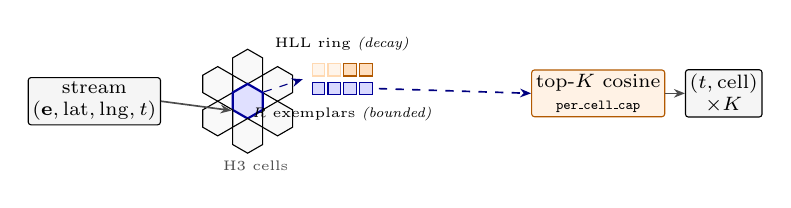
\begin{tikzpicture}[
    >={Stealth[length=1.4mm,width=1.1mm]},
    font=\scriptsize,
    box/.style={draw, rounded corners=1pt, align=center,
                inner sep=1.5pt, minimum height=4.5mm, fill=white},
    iobox/.style={box, fill=gray!8},
    hex/.style={draw, regular polygon, regular polygon sides=6,
                minimum size=4.4mm, inner sep=0pt, rotate=30, fill=gray!5},
    hexhi/.style={hex, fill=blue!12, draw=blue!60!black, thick},
    hllbox/.style={draw, minimum width=1.6mm, minimum height=1.6mm,
                   inner sep=0pt, fill=orange!25, draw=orange!70!black},
    hllold/.style={hllbox, fill=orange!8, draw=orange!30},
    resvslot/.style={draw, minimum width=1.6mm, minimum height=1.6mm,
                     inner sep=0pt, fill=blue!15, draw=blue!60!black},
    flow/.style={->, semithick, gray!60!black},
    smallflow/.style={->, thin, gray!60!black},
]

% ---- streaming input ----
\node[iobox] (in) {stream\\$(\mathbf{e},{\rm lat,lng},t)$};

% ---- H3 hex cluster ----
\coordinate (hexcenter) at ($(in.east) + (11mm, 0mm)$);
\node[hex]   (h0) at ($(hexcenter) + (-3.8mm, 2.2mm)$) {};
\node[hex]   (h1) at ($(hexcenter) + ( 0mm,   4.4mm)$) {};
\node[hex]   (h2) at ($(hexcenter) + ( 3.8mm, 2.2mm)$) {};
\node[hexhi] (hC) at (hexcenter) {};
\node[hex]   (h4) at ($(hexcenter) + (-3.8mm,-2.2mm)$) {};
\node[hex]   (h5) at ($(hexcenter) + ( 0mm,  -4.4mm)$) {};
\node[hex]   (h6) at ($(hexcenter) + ( 3.8mm,-2.2mm)$) {};
\node[font=\tiny, below=4.6mm of hC, gray!60!black] {H3 cells};

% ---- per-cell state pop-out ----
\coordinate (cellAnchor) at ($(hexcenter) + (12mm, 1mm)$);
% HLL ring (top row) with label ABOVE it
\node[hllold] (hll1) at ($(cellAnchor) + (-3mm, 3.0mm)$) {};
\node[hllold] (hll2) at ($(cellAnchor) + (-1mm, 3.0mm)$) {};
\node[hllbox] (hll3) at ($(cellAnchor) + ( 1mm, 3.0mm)$) {};
\node[hllbox] (hll4) at ($(cellAnchor) + ( 3mm, 3.0mm)$) {};
\node[font=\tiny, above=0.3mm of hll2, anchor=south, xshift=1mm]
     {HLL ring \textit{(decay)}};
% Reservoir (bottom row) with label BELOW it
\node[resvslot] (r1) at ($(cellAnchor) + (-3mm, 0.6mm)$) {};
\node[resvslot] (r2) at ($(cellAnchor) + (-1mm, 0.6mm)$) {};
\node[resvslot] (r3) at ($(cellAnchor) + ( 1mm, 0.6mm)$) {};
\node[resvslot] (r4) at ($(cellAnchor) + ( 3mm, 0.6mm)$) {};
\node[font=\tiny, below=0.3mm of r2, anchor=north, xshift=1mm] (rlab)
     {$R$ exemplars \textit{(bounded)}};
\draw[smallflow, dashed, blue!50!black]
     (hC.east) -- ($(cellAnchor) + (-5mm, 1.8mm)$);

% ---- query ----
\node[box, right=24mm of cellAnchor, align=center, fill=orange!10,
      draw=orange!70!black] (topk)
     {top-$K$ cosine\\{\tiny\caponek}};
\node[iobox, right=2.5mm of topk] (out)
     {$(t,{\rm cell})$\\$\times K$};

% ---- flows ----
\draw[flow] (in.east) -- (hC.west);
% reservoir -> top-K: exit right from the reservoir row, clear of labels
\draw[flow, dashed, blue!50!black]
     ($(r4.east)+(0.8mm,0)$) -- (topk.west);
\draw[flow] (topk.east) -- (out.west);

\end{tikzpicture}
\caption{\textbf{\psm{} schematic.} Streaming
$(\mathbf{e},\mathrm{lat},\mathrm{lng},t)$ tuples are deposited into H3
cells; each cell keeps a bounded ring of HLL sketches (orange, fading with
age) and $R$ reservoir-sampled embeddings (blue). A query cosine-searches
the reservoirs under the \caponek{} gate and returns $K$ cell-tagged
candidates. State is bounded per cell, independent of recording length.}
\label{fig:f1-schematic}
\end{figure}


% P3: HDD multi-session results — the core payload. Adapted from the 8pp
% §5.6; cross-refs to supp/limitations rewritten to be self-contained.

\section{Multi-Session Persistence at Metropolitan Scale}
\label{sec:results-hdd}

We evaluate on the Honda Research Institute Driving Dataset
(HDD)~\cite{ramanishka2018hdd}: 104\,h of San Francisco Bay Area driving
with RTK GPS and a front camera (our extraction covers 132 drives,
102.9\,h with valid GPS). Over 8 months a vehicle genuinely re-drives the
same streets. HDD ships no look-back-QA labels, so these results are
\emph{systems} and \emph{self-supervised}, not retrieval-accuracy; frames
are embedded with CLIP-L.

\paragraph{Revisit structure.}
Binning every drive to H3 $r{=}10$ (${\sim}66$\,m), \textbf{47.0\%} of
(drive, cell) traversal events fall in cells revisited on $\geq2$ distinct
days (pre-registered bar: $\geq30\%$), across 5{,}163 revisited cells
whose first-to-last visit spans a \textbf{median of 106 days} (max 221);
the coverage is arterial, not a depot artifact (46.5\% excluding the 20
most-driven cells).

\paragraph{State scales with area, not time (Fig.~\ref{fig:hdd-combined}A).}
Over 102.9\,h and 23{,}298 distinct $r{=}10$ cells, \psm{}'s
per-cell-capped state ($\sum_\text{cells}\min(\text{frames}, R)$) is
smaller than a dense per-frame bank at every ingest rate, the gap widening
as the reservoir caps redundant dwell/revisit frames:
$1.3\times$/$2.3\times$/$4.3\times$/$7.2\times$ at 1/5/15/30\,fps (capping
26/57/77/86\% of frames)---state grows \emph{sublinearly in observation
count}, $O(\text{distinct cells})$ not $O(\text{frames})$. This is not a
plateau (area keeps growing: only 20\% of cells seen by the halfway mark);
the saving is per-cell capping, the empirical form of ``budgeted by area,
not sequence length.''

\paragraph{Cross-session cardinality accrual and decay
(Fig.~\ref{fig:hdd-combined}B).}
HDD's revisits exercise the HLL sketch \emph{across sessions}. Feeding a
revisited cell's frames chronologically across drives, a single fixed
$1\,\mathrm{KiB}$ ($p{=}10$) sketch accrues to \textbf{8{,}112 unique
observations over 219 days} while its 60-slot ring-buffer windowed estimate
decays between visits and jumps on each revisit; a Python reimplementation
matches the C-engine sketch to $2.4\times10^{-5}$ median relative error.

\paragraph{The persistent memory is retrievable across sessions
(Fig.~\ref{fig:hdd-combined}C).}
Label-free, we query a revisited cell with a drive-A exemplar and measure
the AUC that different-day drive-B frames in that cell outrank frames from
other cells. Over 5{,}222 revisited cells with valid cross-drive pairs
(2{,}000 stratified queries) the cross-session AUC is \textbf{0.853}, vs.\
a shuffled-cell null of $0.498$ and a same-drive upper bound of $0.977$---
strong cross-session place recognition from CLIP cosine over the persistent
per-cell exemplars alone. The same-cell-vs-all-others split blends
geographic proximity with visual identity; a $k$-nearest-cell control would
isolate the latter.

\begin{figure}[t]
\centering
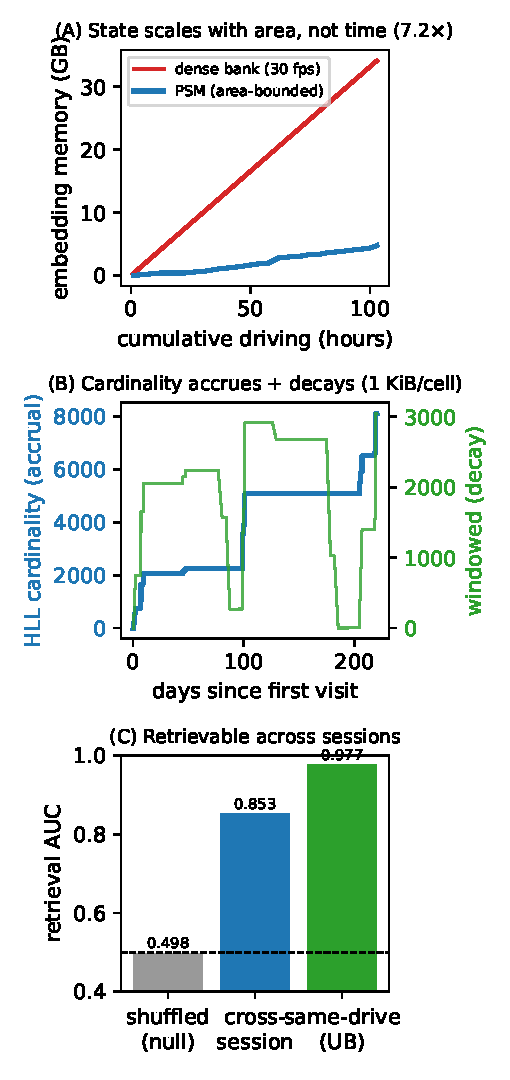
\includegraphics[width=0.86\linewidth]{figures/hdd_combined.pdf}
\caption{HDD multi-session results (132 drives, 102.9\,h).
\textbf{(A)}~\psm{}'s area-bounded per-cell reservoir vs a dense per-frame
embedding bank over cumulative driving hours; the gap widens with ingest
rate as redundant frames are capped ($O(\text{cells})$, not
$O(\text{frames})$; drawn at 30\,fps).
\textbf{(B)}~Cross-session HLL cardinality on the most-revisited cell:
cumulative accrual (left axis) in a fixed $1\,\mathrm{KiB}$ sketch, and the
ring-buffer windowed estimate (right axis) decaying between visits and
jumping on each revisit, over months-long gaps.
\textbf{(C)}~Self-supervised cross-session retrieval AUC (different-day
same-cell frames outranking other-cell frames), with the shuffled-cell
null ($0.498$) and same-drive upper bound ($0.977$).}
\label{fig:hdd-combined}
\end{figure}

% P4: retrieval-fidelity validation (inline, no table), generalization
% pointer, limitations (3 sentences), conclusion + MIT.

\section{Retrieval Fidelity and Scope}
\label{sec:validation}

\paragraph{The substrate does not lose recall.}
Bounding memory is only useful if retrieval survives it. On a wearable
look-back-QA corpus (Nymeria~\cite{ma2024nymeria} atomic-action
narrations), \psm{} at the eviction-free operating point recovers
brute-force CLIP retrieval \emph{exactly} (the same 25 of 187 groundable
narrations at identical mean IoU) and at the bounded $R{=}128$ deployment
point reaches 83\% of brute-force Hit@5 at $8\times$ smaller per-cell
state; with a single MLLM rerank the strict-diversity point matches
brute-force on localization within sampling noise. The spatial-axis
behavior further holds across 14 street-scale sessions spanning three
sensor stacks (SLOPER4D~\cite{dai2023sloper4d}, Nymeria,
LookOut~\cite{pan2025lookout}) and three encoders (CLIP-L, CLIP-bigG,
SigLIP-2~\cite{tschannen2025siglip2}); the full generalization study,
ablations, and MLLM comparison are deferred to the extended paper.

\paragraph{Limitations and outlook.}
The HDD results are systems and self-supervised, not a retrieval-accuracy
metric, since HDD carries no QA labels; the cross-session AUC conflates
geographic proximity with visual identity pending a $k$-nearest-cell
control. Reported latency is host-CPU, not on-device, and the extracted
HDD features carry a ${\sim}3$\,s GPS-warmup skew (${\sim}17$\,m) corrected
at analysis time (shifting AUC by $+0.005$). Nonetheless, by budgeting
spatial memory by area rather than time---bounded per-cell state,
time-decayed HLL cardinality, and reservoir exemplars under a \caponek{}
knob---\psm{} demonstrates on 102.9\,h of driving the multi-session
regime a single-pass corpus cannot: sublinear state growth, cross-session
cardinality accrual with decay, and label-free cross-session place
recognition, while matching brute-force retrieval at bounded memory on a
wearable corpus. The engine and harness are released under
MIT.\footnote{Repository URL withheld for double-blind review.}


\bibliographystyle{splncs04}
\bibliography{references}

\end{document}
